\documentclass[11pt]{beamer}
\usetheme{Pittsburgh}
\usepackage[utf8]{inputenc}
\usepackage[spanish]{babel}
\usepackage{amsmath}
\usepackage{amsfonts}
\usepackage{amssymb}
\usepackage{graphicx}
\author{Luis Greco - Marcela Herrera - Cristian Kubrak - Alejo Salvador }
\title{Trabajo Práctico 3}
\subtitle{Tomografía computada}
%\setbeamercovered{transparent} 
%\setbeamertemplate{navigation symbols}{} 
%\logo{} 
%\institute{} 
%\date{} 
%\subject{} 
\begin{document}



\begin{frame}
\titlepage 
\end{frame}


\begin{frame}{INTRODUCCIÓN}
\begin{itemize}
\item El objetivo de este trabajo práctico es evaluar un método para reconstruir imágenes tomográficas sujetas a ruido, utilizando el método de aproximación por cuadrados mínimos.
\end{itemize}
\end{frame}

\begin{frame}{PREMISAS}
\begin{itemize}
\item Nuestro sujeto es una imagen de $n$x$n$ pixeles discretizada en celdas de $d$x$d$ pixeles.
\item La intensidad de un pixel se asocia al tiempo que demora un rayo en atravesar ese pixel.
\item La distancia que recorre un rayo que atraviesa al sujeto es igual a la cantidad de pixeles por los que pasa.
\item En cinemática $Velocidad = Espacio/Tiempo$. En este caso la ''velocidad'' promedio dentro de la celda $k$ es:
\begin{displaymath}
v_{k} =(\sum_{i=1}^{n}\sum_{j=1}^{n} I_{[i][j]})/n*n
\end{displaymath}
\item Los rayos están sujetos a ruido.
\end{itemize}
\end{frame}


\begin{frame}{DESARROLLO}
\frametitle{Distancia recorrida por un rayo}
\end{frame}

\begin{frame}
\frametitle{Velocidad de un rayo}
\end{frame}

\begin{frame}
\frametitle{Generación de rayos}
\begin{figure}[H] 
\centering
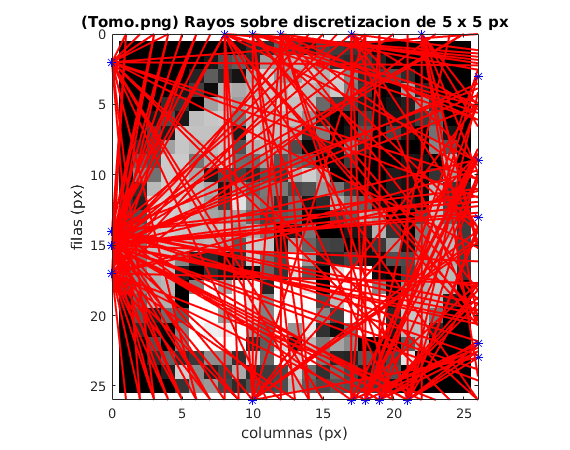
\includegraphics[scale=0.5]{img/rayos_tomo25x25px.png}
\caption{Trazado aleatorio de rayos}
\label{fig:rayos aleatorios}
\end{figure}

\framesubtitle{Cantidad y ubicación de los emisores}

\end{frame}


\begin{frame}
\frametitle{Ruido}
\end{frame}


\begin{frame}

\end{frame}

%\begin{frame}
%\tableofcontents
%\end{frame}

\begin{frame}{Carátula}
\begin{itemize}

\item Como no tenemos un tomógrafo a disposición partimos de imágenes tomográficas reales en formato 16 bits, las discretizamos y utilizamos las intensidades de los pixeles como una medida del tiempo que le toma a un rayo atravesar el pixel.
\item Simulamos rayos X que atraviesan la imagen.
\item Una vez generados los rayos se calculan las ''velocidades'' de cada celda de la cuadrícula utilizando el método de cuadrados mínimos lineales. \item Se evalúan los resultados obtenidos usando error cuadrático medio.
\item Por último se reconstruye la imagen a partir de los datos calculados en formato pgm de 8 bits.
\end{itemize}
\end{frame}

\end{document}

